\addcontentsline{toc}{chapter}{Appendices}

% The \appendix command resets the chapter counter, and changes the chapter numbering scheme to capital letters.
%\chapter{Appendices}
\appendix
\chapter{Plotppendix}
\label{Plotpend}
This appendix hold the additional plots and tables that provide contextual information useful but not essential for understanding the project.  


\section{Additional plots}

\begin{figure}
    \centering
    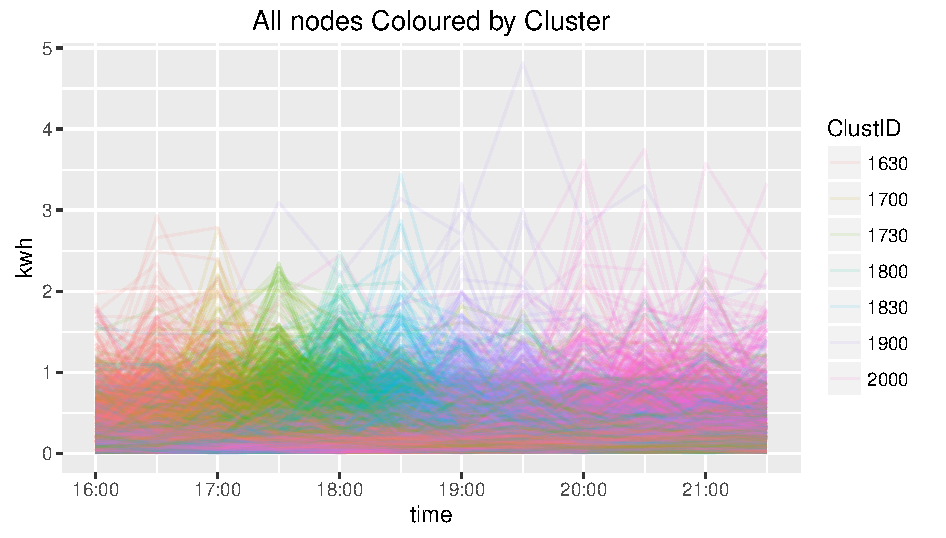
\includegraphics[width = \textwidth]{Figures/Appendix/AllNodesClustercolour}
    \caption[All Nodes for one day]{The distinct cluster forms can be seen across all the clusters, the soup node has no pattern and is clearly just noise.}
    \label{fig:AllNodesClustercolour}
\end{figure}


\begin{figure}
    \centering
    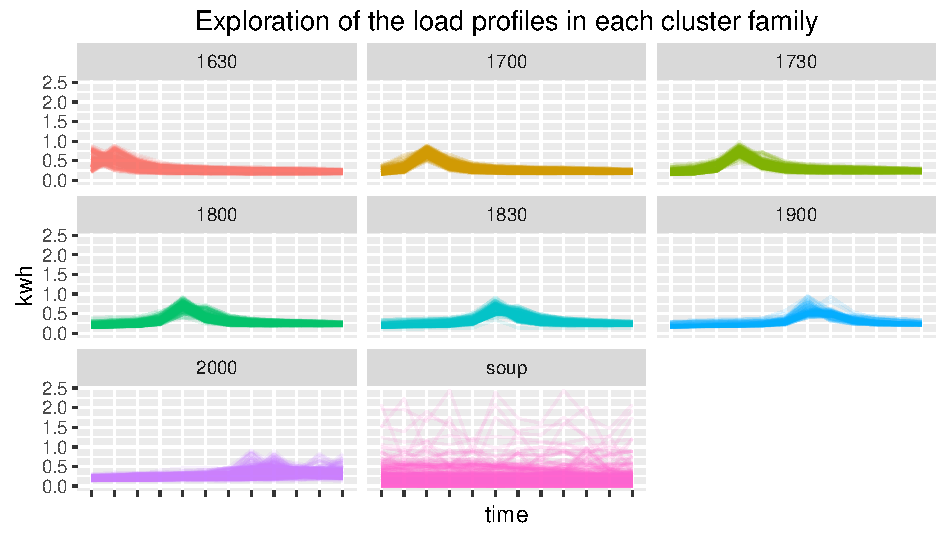
\includegraphics[width = \textwidth]{Figures/Appendix/AllCLustFamilies}
    \caption[All Clusters grouped by family]{The distinct cluster forms can be seen across all the clusters, the soup node has no pattern and is clearly just noise.}
    \label{fig:AllCLustFamilies}
\end{figure}

\section{Additional tables}
% latex table generated in R 3.3.0 by xtable 1.8-2 package
% Wed Aug 17 16:25:24 2016
\begin{table}[ht]
\centering
\begin{tabular}{rlrrrrrrrr}
  \hline
 & ClustID & 1630 & 1700 & 1730 & 1800 & 1830 & 1900 & 2000 & soup \\ 
  \hline
1 & 1630 & 0.31 & 0.13 & 0.09 & 0.09 & 0.08 & 0.06 & 0.22 & 0.01 \\ 
  2 & 1700 & 0.23 & 0.17 & 0.12 & 0.11 & 0.08 & 0.06 & 0.22 & 0.01 \\ 
  3 & 1730 & 0.18 & 0.13 & 0.16 & 0.13 & 0.10 & 0.06 & 0.23 & 0.01 \\ 
  4 & 1800 & 0.16 & 0.11 & 0.13 & 0.16 & 0.12 & 0.07 & 0.24 & 0.01 \\ 
  5 & 1830 & 0.16 & 0.09 & 0.10 & 0.13 & 0.14 & 0.09 & 0.28 & 0.01 \\ 
  6 & 1900 & 0.16 & 0.09 & 0.09 & 0.10 & 0.13 & 0.12 & 0.31 & 0.01 \\ 
  7 & 2000 & 0.15 & 0.09 & 0.08 & 0.09 & 0.10 & 0.08 & 0.40 & 0.01 \\ 
  8 & soup & 0.20 & 0.09 & 0.08 & 0.10 & 0.09 & 0.06 & 0.24 & 0.14 \\ 
   \hline
\end{tabular}
\caption{The cluster transition probabilities} 
\label{tab:clustrans}
\end{table}


\chapter{Visualising Large Data Sets Using Aggregated Heatmaps}
\label{app:heatmaps}

\chapter{Community distance}
\label{community distance}

An interesting question to consider is the graph distance between two communities that share no common nodes. This is interesting because if two graphs share no common nodes then intuitively they shouldn't be in the same cluster of communities. Although solving this problem is beyond the scope of this project, the discussion below describes some cases and shows that probability of randomly moving from y to x decreases exponentially with a linear increase in additional connected clusters.

In this section communities will be represented as nodes which are made up of a binary vector of length l (each element representing a node in the original graph ), the edges of the graph are defined by the Jaccard similarity coefficient (JSC) betwen the node vectors. A JSC of 0 means no edge for any other value, the edge distance is the JSC and it's probability weight is the normalised inverse JSC. This  is shown in equations \ref{eq:JSC} and \ref{eq:JSCdist}. In this context the distance graph is undirected and the graph of weighted probabilities is directed.

\begin{equation}
    J(A,B)=\frac{A\cap B}{A\cup B}=JSC
    \label{eq:JSC}
\end{equation}


\begin{equation}
    \frac{1}{JSC}=\frac{A\cup B}{A\cap B}=Dist
    \label{eq:JSCdist}
\end{equation}


\section{Question 1:} When there are three nodes in the network what is the minimum distance between nodes $x$ and $y$, a schematic of this graph can be seen in \ref{net:threenodes}

\begin{figure}[ht]
    \centering
    \includestandalone{Tikz/CommDist/threenodes}
    \caption[Three Node graph]{Three node setup, showing the relationships within the network.}
    \label{net:threenodes}
\end{figure}

As it is stated that$x_1 \notin y$, then $ y\cup S \supset y $ as $S$ must have at least 1 element of $x$ as a result $K \cup S$ (K is either of the none overlapping sets) is a proper superset of both $y$ and $x$. Fully defined $K \cup S = y \cup x \cup z$ where $z$ are all elements that are not members of either $y$ or $x$, giving in total 3 non overlapping sets.

Therefore to minimise the distance from node y to S, $y \cap S$ needs to be maximised. This occurs when the entire of $y$ is found in vector $S$ making the resulting JSC between the two nodes. 

\begin{equation}
    \frac{|y|}{|x|+|y|+|z|}
\end{equation}

and the distance

\begin{equation}
    \frac{|x|+|y|+|z|}{|y|}
\end{equation}

The distance between $x$ and $y$ is then

\begin{equation}
    \frac{|x|+|y|+|z|}{|y|} +\frac{|x|+|y|+|z|}{|x|} = 2 + \frac{|z|}{|x|+|y|}+\frac{|x|^2+|y|^2}{|x||y|}
\end{equation}

Which is minimised when $z=0$ and $|x|=|y|$ making the minimum distance between two non-overlapping nodes separated by a common node 4 as shown below


\begin{equation}
    4 =2 + \cancel{\frac{0}{|x|+|x|}}+\frac{|x|^2+|x|^2}{|x||x|} =2+\frac{2\cancel{|x|^2}}{\cancel{|x|^2}}
\end{equation}


The resulting weighted graph can be seen in figure \ref{net:weight3nodes}

\begin{figure}
    \centering
    \includestandalone{Tikz/CommDist/weighted3nodes}
    \caption[Three Node directed graph]{The Weighted directional graph shows the probability of moving from 1 node to another}
    \label{net:weight3nodes}
\end{figure}

\section{Question 2:}
Building on the previous section the effect on probability of of moving from y to x is considered with more than one connecting node. What is the probability of having arrived at node x by time t or earlier given n nodes where $S=S_n$?

To begin this problem, the previous problem can be considered with two overlapping nodes (where $S_1=S=2$) instead of 1. Figure \ref{net:4nodes} shows the construction of such a graph and that the distance between the identical nodes is 1 as would be expected when using inverse Jaccard distance.


\begin{figure}[ht]
    \centering
    \includestandalone{Tikz/CommDist/fournodes}
    \caption[Four node graph]{Weighted undirected graph shows the distance between the nodes of the network when there are two identical joining nodes.}
    \label{net:4nodes}
\end{figure}



The extension of figure \ref{net:4nodes} is to increase from 2 to n identical connecting nodes. The number of edges connecting x and y to the S nodes are n each, the number of edges connecting the S nodes with each other follows the triangle number series $E=\frac{(n-1)n}{2}$. As the S nodes are all identical they can be represented as a simplified directed weighted graph as shown in figure \ref{net:Nnodesweighted}. The derivation of the weights is shown in equations \ref{eq:unormweights} to \ref{eq:stayinS}.

\begin{figure}[ht]
    \centering
    \includestandalone{Tikz/CommDist/Nnodes}
    \caption[N node unweighted Graph]{This undirected graph shows all the edges of a network of n+2 nodes where 2 two nodes have no overlap and n nodes are identical and whose make up means the distance between x and y is minimised. Distances have not been included but are similar to figure \ref{net:4nodes} in that links to the S nodes are length 2 and between S nodes are length 1}
    \label{net:Nnodes}
\end{figure}


\begin{figure}[ht]
    \centering
    \includestandalone{Tikz/CommDist/Nweighted}
    \caption[N node transfer probability]{Weighted directed graph shows the probability of transfer between nodes in the network when there are n identical joining nodes that make up the set S. There is no arrow back from x as once the random process has reached x the process halts.}
    \label{net:Nnodesweighted}
\end{figure}

The sum of unormalised weights of S are 
\begin{equation}
    \frac{2+(n-1)n}{2}= \frac{1}{2}+\frac{1}{2}+\frac{(n-1)n}{2}= 1+\frac{(n-1)n}{2}
    \label{eq:unormweights}
\end{equation}

Using this as a normalisation constant probability of transferring from S to either x or y is 
\begin{equation}
    \frac{1}{2+(n-1)n}=\frac{\frac{1}{\cancel{2}}}{\frac{2+(n-1)n}{\cancel{2}}}
\end{equation}

The normalised probability of stay in in the S is given by
\begin{equation}
        \frac{(n-1)n}{2+(n-1)n}=\frac{\frac{(n-1)n}{\cancel{2}}}{\frac{2+(n-1)n}{\cancel{2}}}
        \label{eq:stayinS}
\end{equation}

\chapter{Smart Meters used in the Project}
\label{app:smartmeters}

\chapter{UK domestic Energy breakdown}
\label{sec:Energybreakdown}
Breaking down the domestic energy mix of the UK \cite{domesticenergyv2pdfwithnotes2005} provides more insight into why there could be the low correlations found in \ref{sec:basicconsum}. Overall the majority of UK domestic energy comes from gas, as shown in figure \ref{fig:DomElConsumFuel}, which which makes up over 70\% of the mix compared to 20\% from electricity. Across all fuel types the majority of energy is used on Space heating and water heating which accounts for more than 80\%. When looking at only electricity consumption over 60\% of electricity is used on lighting and appliances with very little on heating. The result is that turning on lights, TV's or computers will have a major effect on consumption, even though they are small relative to the base load of energy consumption overall. This supports the finding of low levels of correlation within a smart meter a minor changes in unimportant object of electricity consumption will have a major effect on the evening behaviour pattern introducing variability.

\begin{figure}
    \centering
    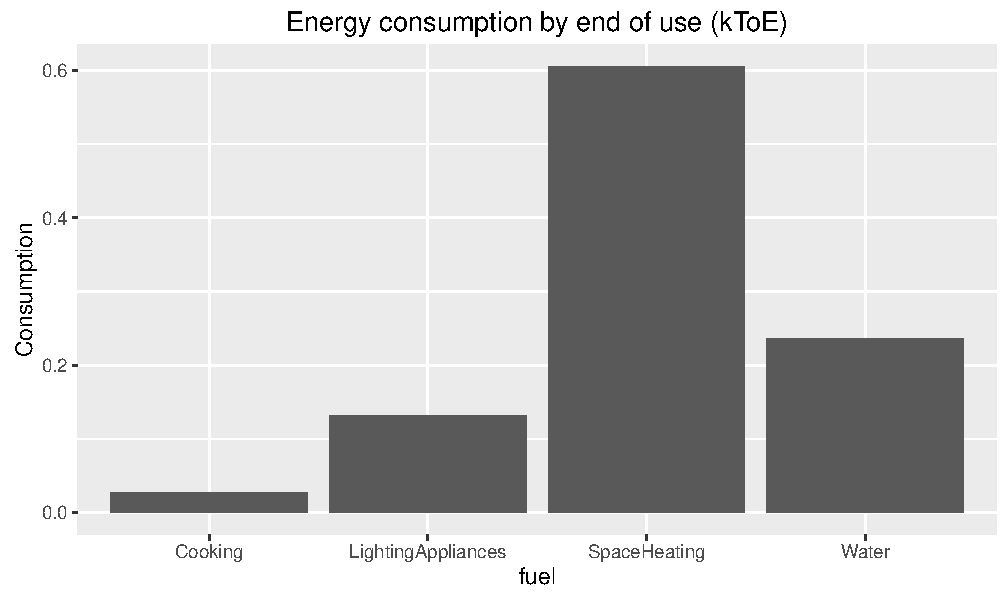
\includegraphics[width =\textwidth]{Figures/Appendix/DomConsumType}
    \caption[Domestic energy consumption by end of use]{Breaking down UK domestic energy consumption by end use across all fuel types it is clear that heating (the combination of SpaceHeating and Water), is the single biggest use of energy consumping over 84\% of all domestic electricity.}
    \label{fig:DomConsumType}
\end{figure}

\begin{figure}
    \centering
    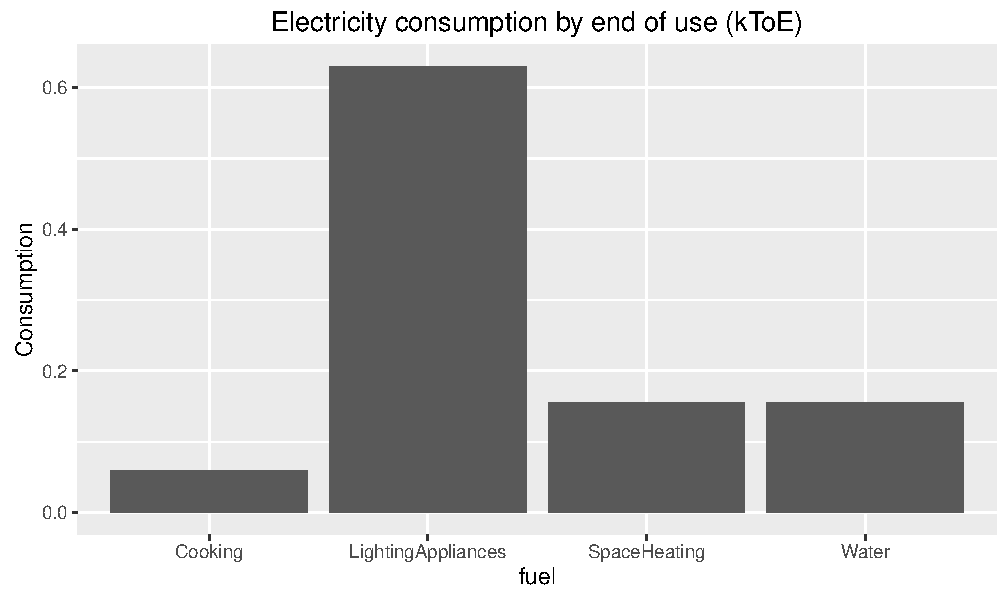
\includegraphics[width =\textwidth]{Figures/Appendix/DomElConsumType}
    \caption[Domestic electricity consumption by end of use]{Breaking down domestic electricity use by end of use shows that the single biggest use of electricity in the home is lighting and Appliances, this contrasts strongly with figures \ref{fig:DomConsumType} overall breakdown of electricity use}
    \label{fig:DomElConsumType}
\end{figure}

\begin{figure}
    \centering
    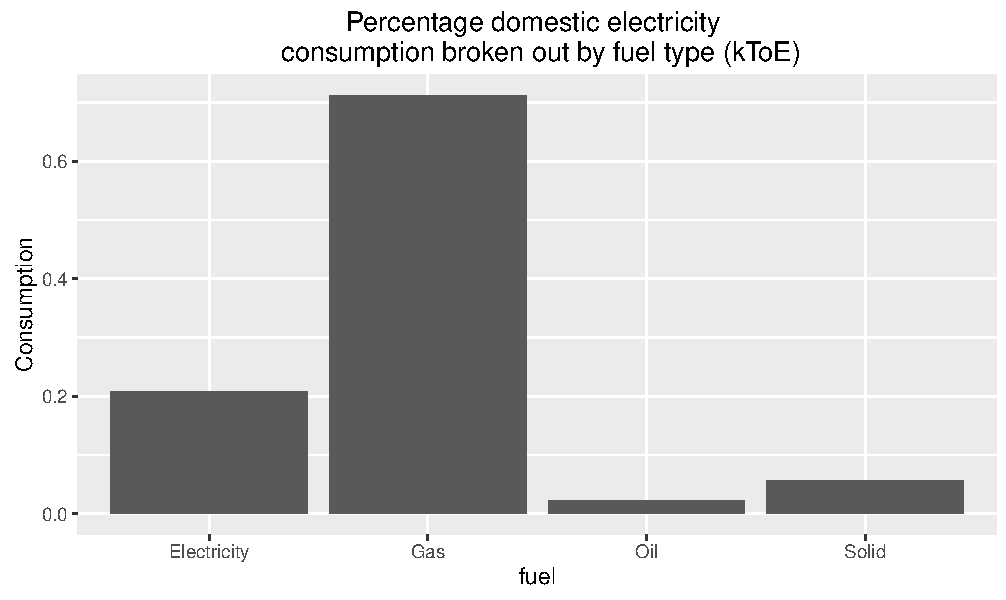
\includegraphics[width =\textwidth]{Figures/Appendix/DomElConsumFuel}
    \caption[Energy consumption by fuel type]{The breakdown of energy fuel types shows that electricity is only 20\% of the total fuel mix gas being about 70\% of total energy consumption.}
    \label{fig:DomElConsumFuel}
\end{figure}

\iffalse
\chapter{Flow Chart of Data process}
The flow charts in this section provide a visual representation of how the project was performed, figure \ref{fig:CleanFlow} shows how the data set TC1a was manipulated so that the the most high quality segments of the data were included and the remaining NA's filled. Figure \ref{fig:ProcessFlow} goes from the cleaning stage, and shows how the data is processed so that it the transition matrix and predictive model can be made and tested. The combination of both figures therefore gives a high level overview of the project from start to finish.

\begin{landscape}

\begin{figure}[ht]
    \centering
    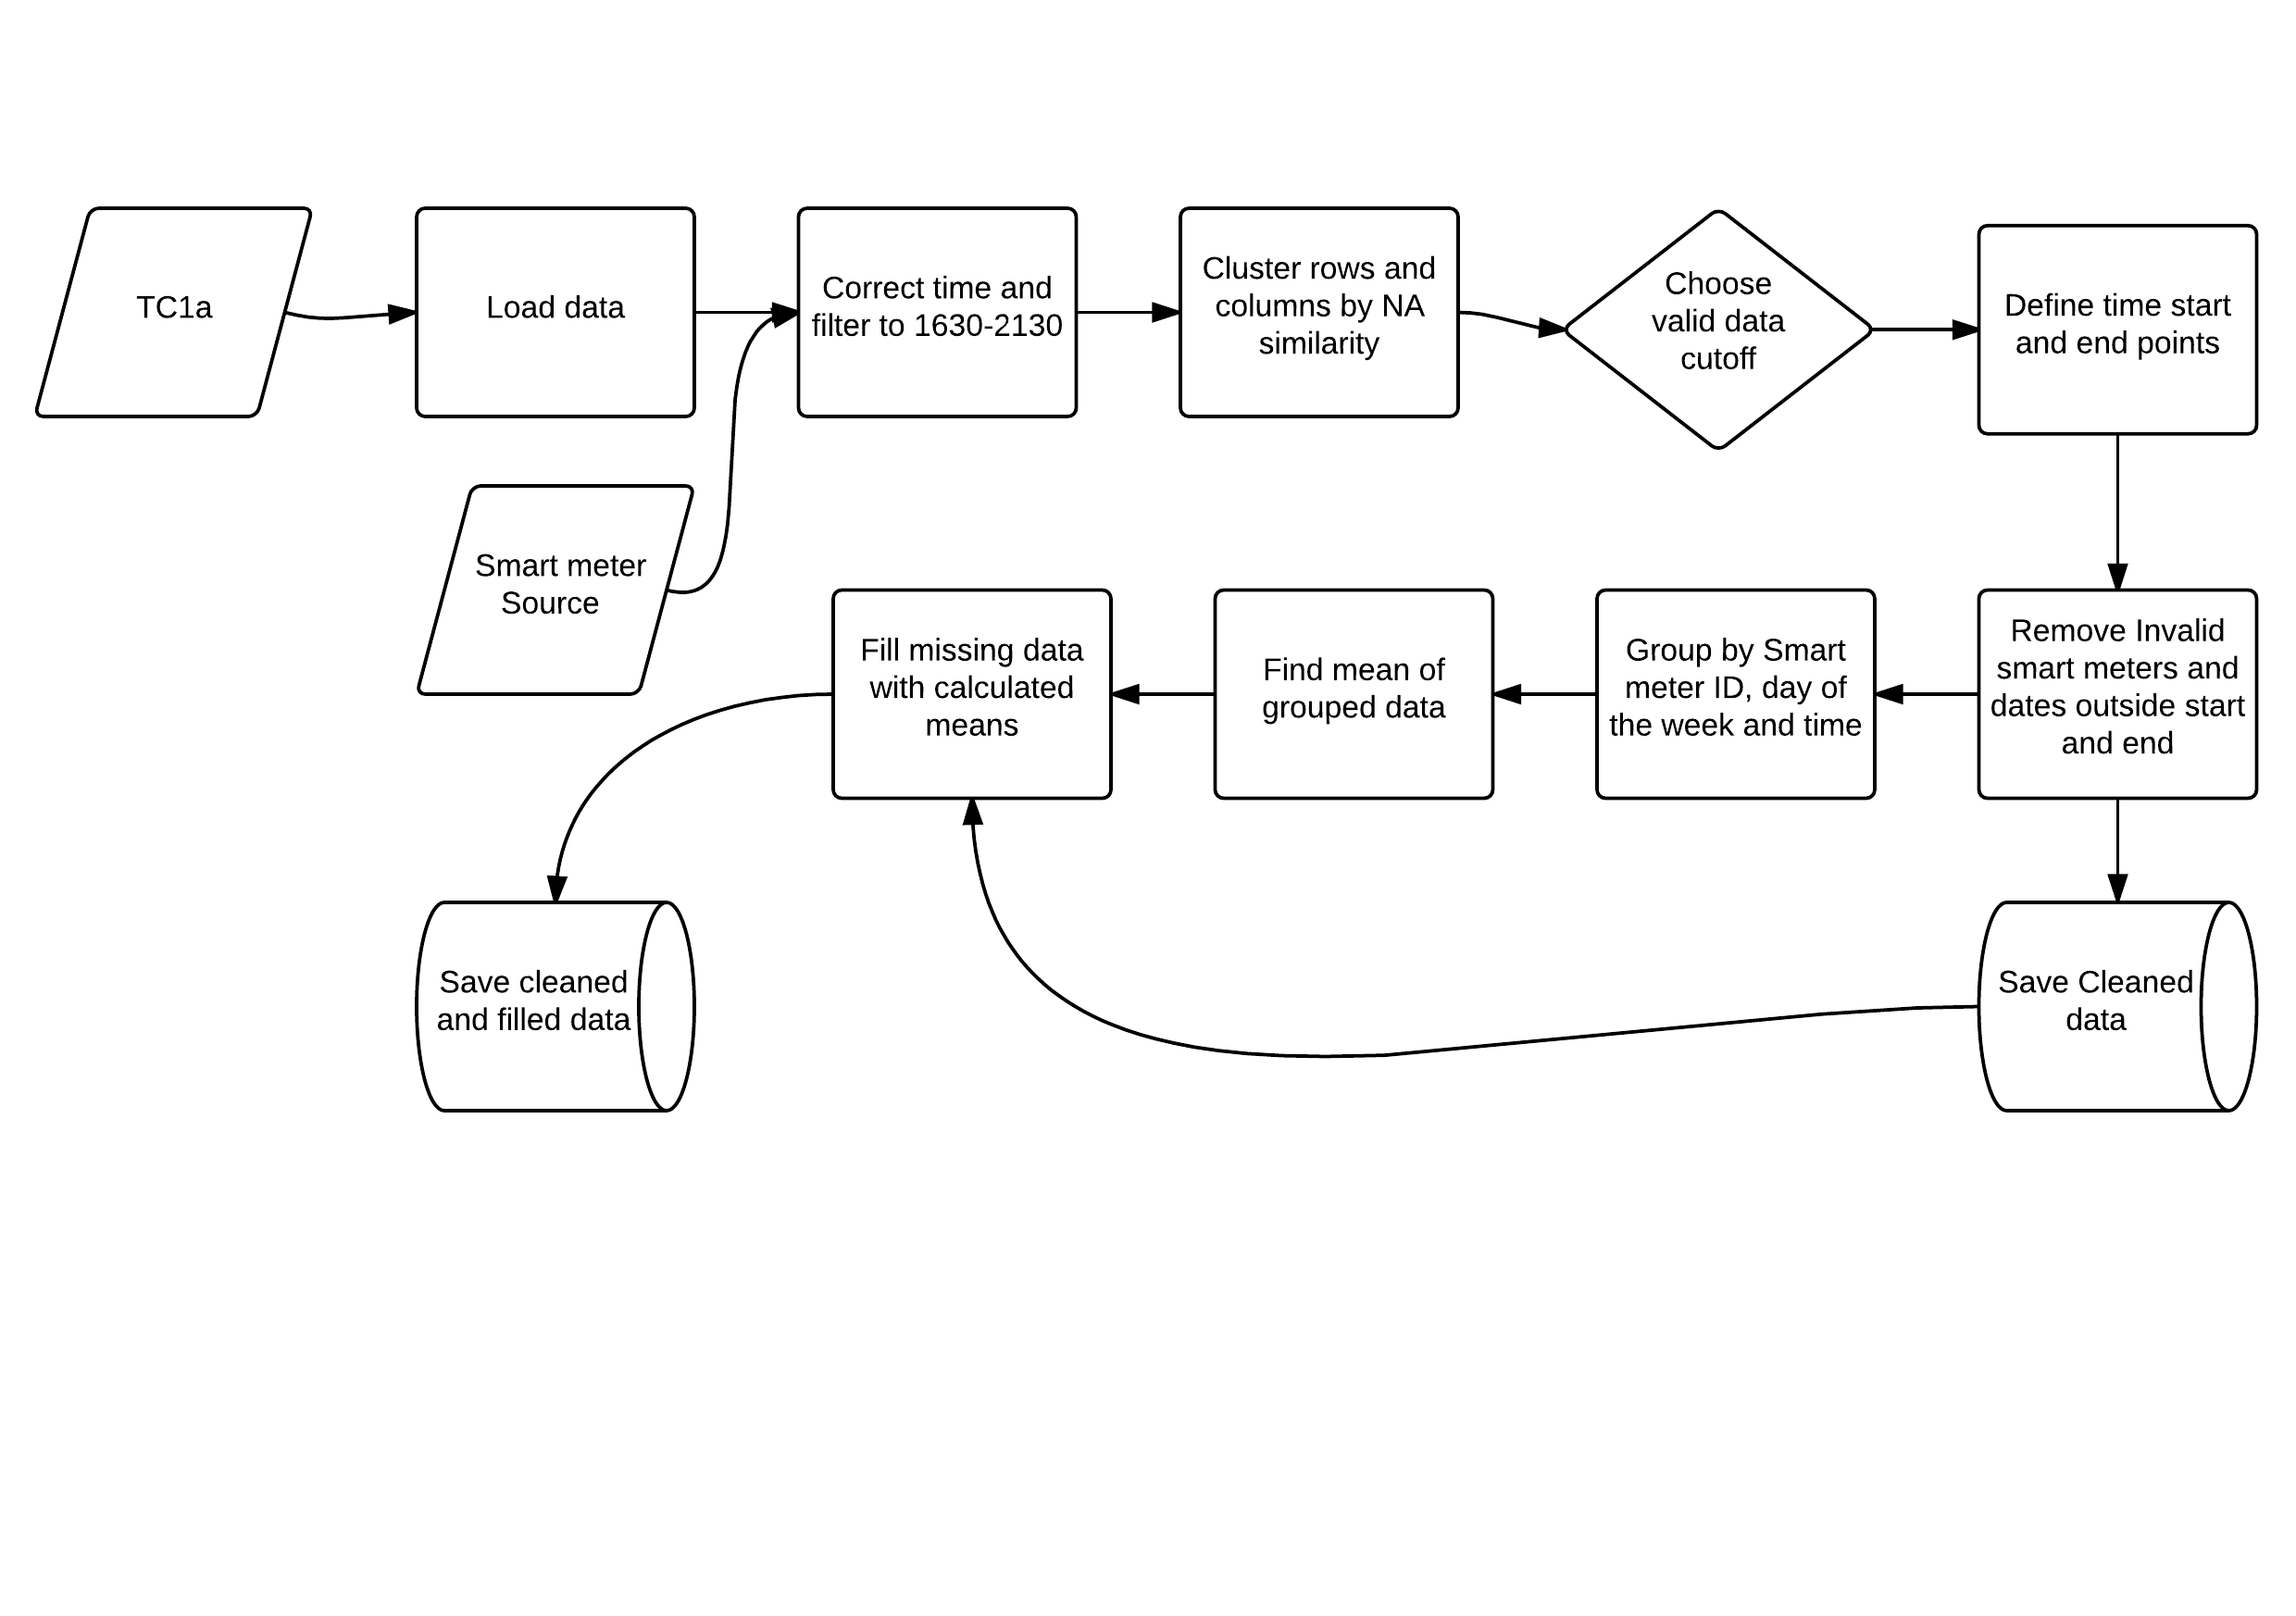
\includegraphics[width =\textwidth]{Figures/Appendix/DataCleaning.png}
    \caption[Data cleaning process]{Flow chart of the Data Cleaning Process}
    \label{fig:CleanFlow}
\end{figure}


\begin{figure}[ht]
    \centering
    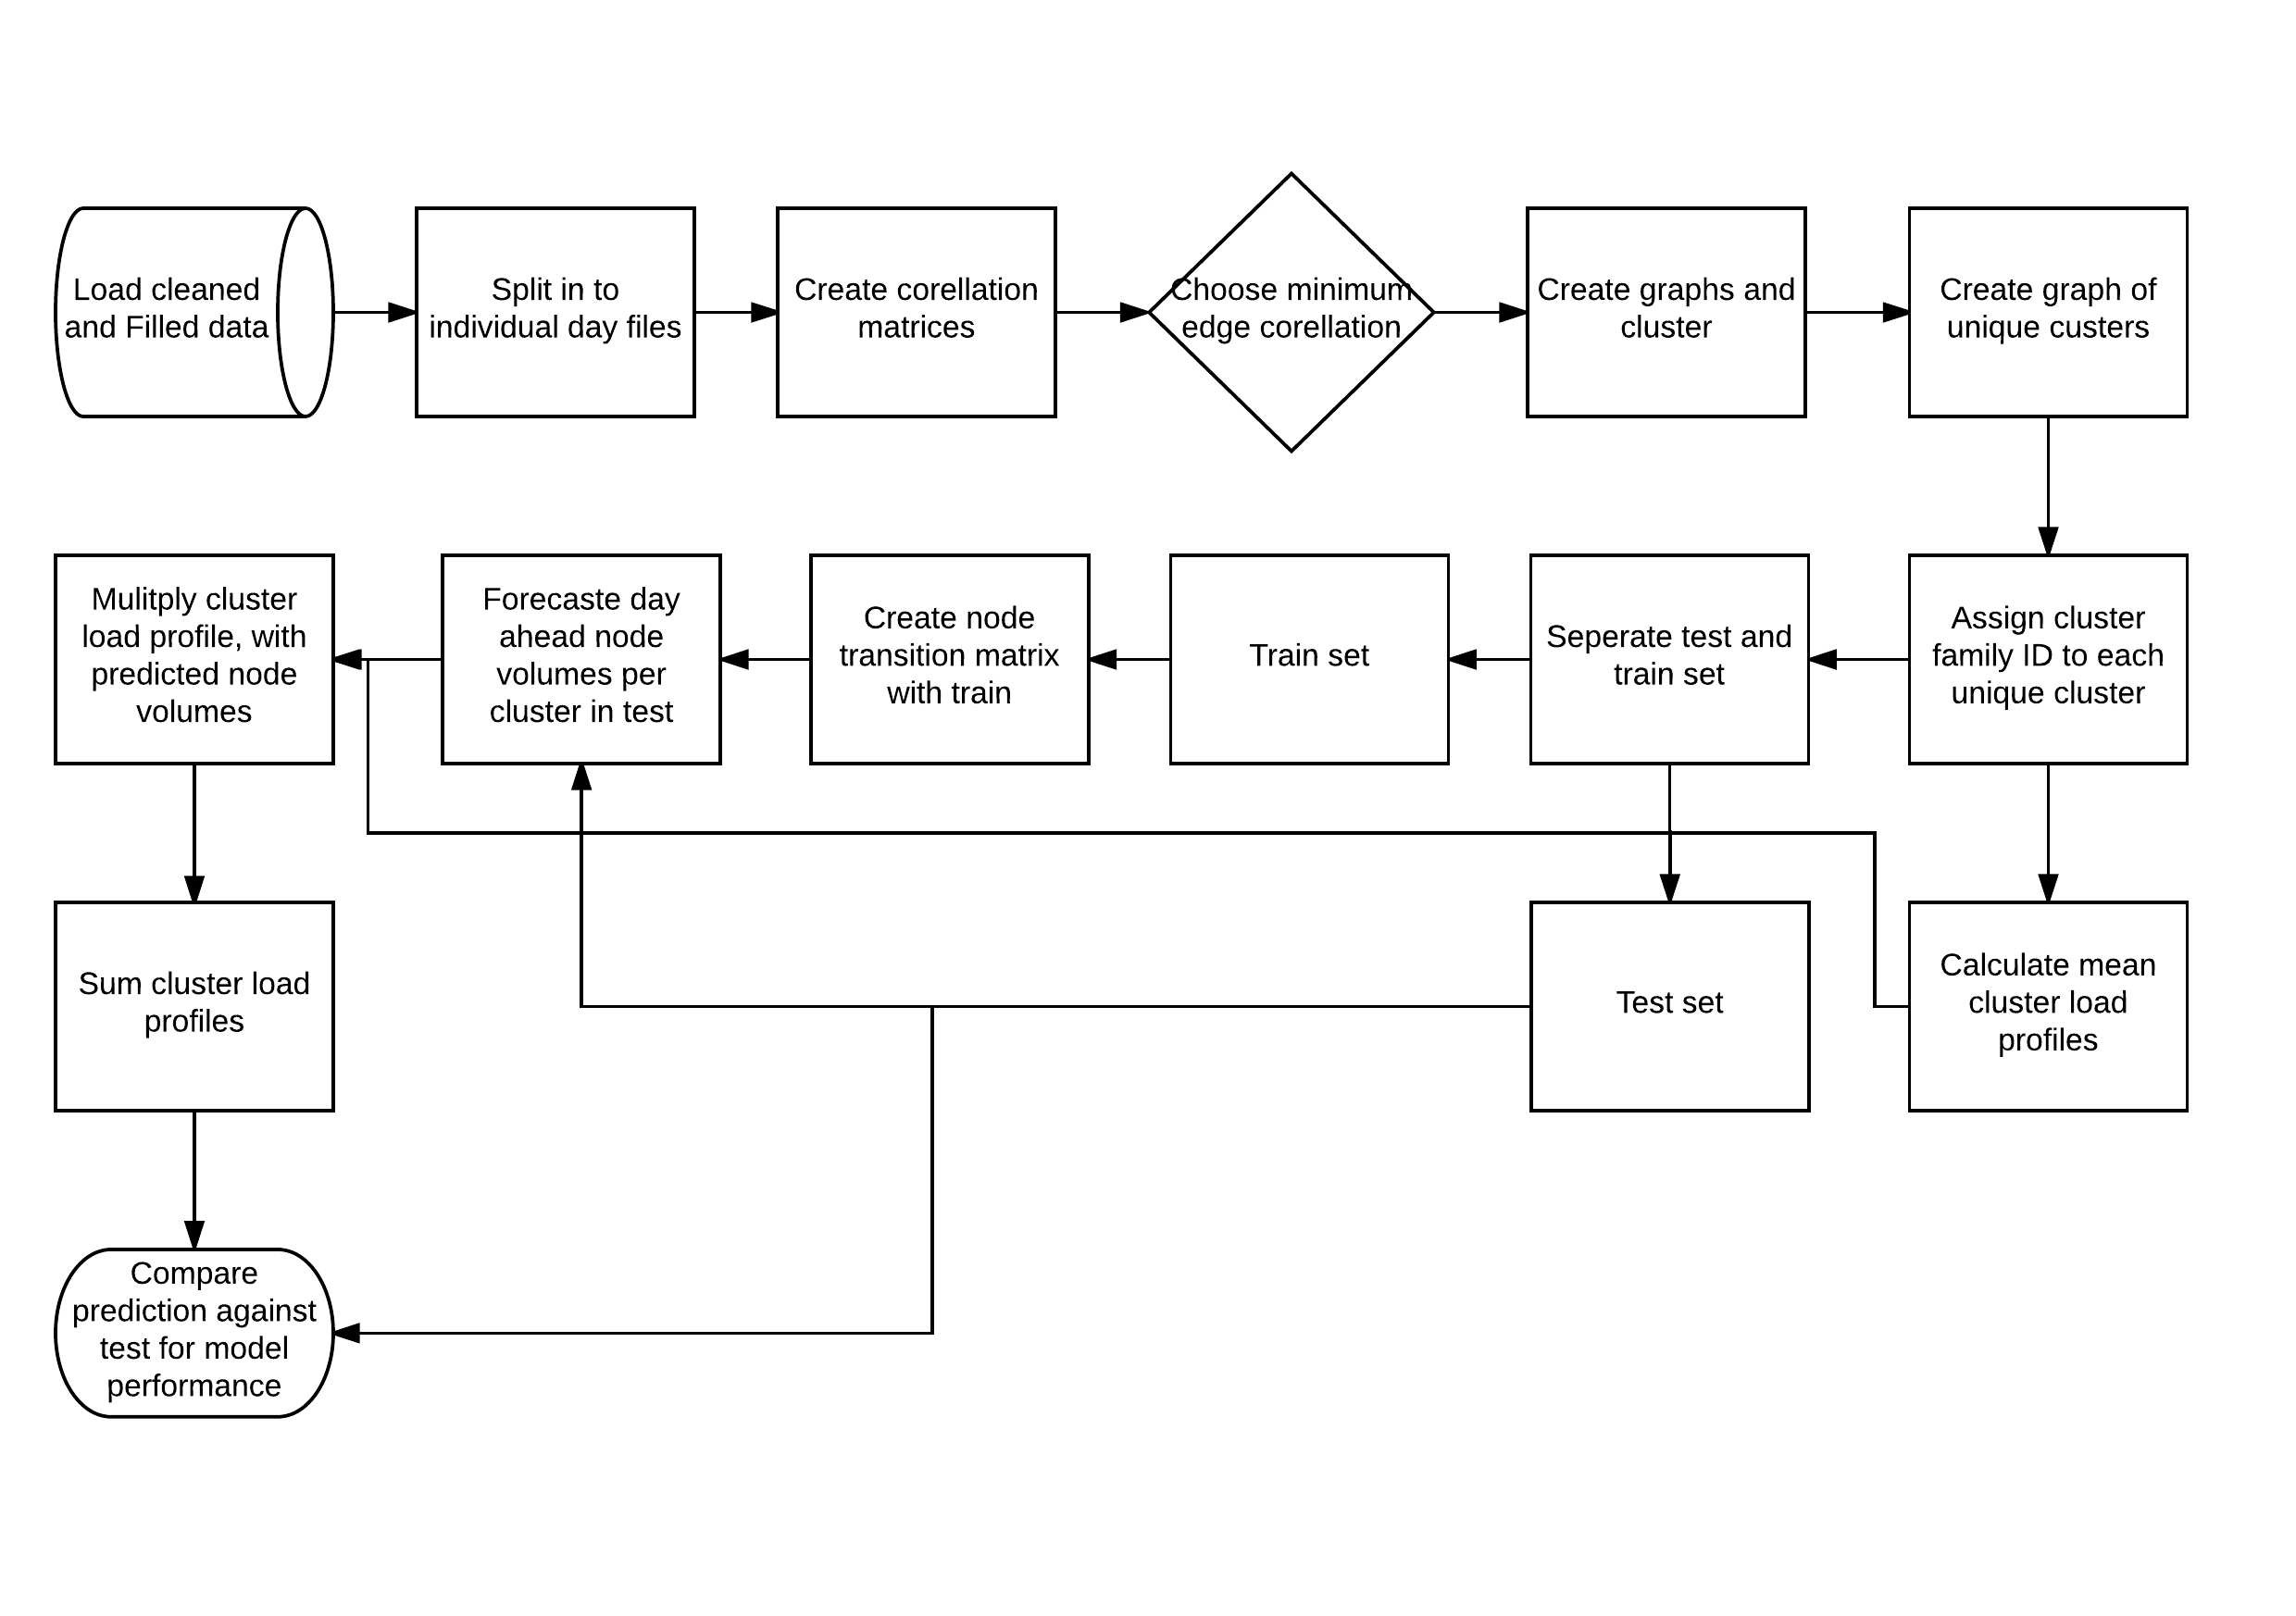
\includegraphics[width =\textwidth]{Figures/Appendix/Thesisprocess.png}
    \caption[Project process]{Flow chart showing the process of generating and testing the predictive model once the data has been cleaned}
    \label{fig:ProcessFlow}
\end{figure}


\end{landscape}
\fi

\chapter{Colophon}
\label{appendixlabel3}
This document was set in the Times Roman typeface using \LaTeX\ and Bib\TeX , composed with ShareLaTeX using the UCL thesis template developed by Ian Kirker. Template Sourcecode can be obtained either through the ShareLaTeX setup wizard or on \href{https://github.com/UCL/ucl-latex-thesis-templates/blob/master/Main.tex}{UCL's Github account}.
The compilable script for this full thesis can be found at \href{https://github.com/JonnoB}{Jonathan Bourne's Github account}. For sharpness, images were imported as PDF files, or if that was not possible as PNG's. All figures were made using R's ggplot2 package, graphs were visualised using either igraph \cite{csrdi2006} or Gephi \cite{bastian2006}.
 % description of document, e.g. type faces, TeX used, TeXmaker, packages and things used for figures. Like a computational details section.
% e.g. http://tex.stackexchange.com/questions/63468/what-is-best-way-to-mention-that-a-document-has-been-typeset-with-tex#63503

% Side note:
%http://tex.stackexchange.com/questions/1319/showcase-of-beautiful-typography-done-in-tex-friends

\chapter{Computational Details}
\label{TechComp}

Computation was performed using cloud computing was performed on amazon EC2 instance. 
The specifications of the instance was scaled according to computational requirements of the specific operation being performed but mostly using the instance shown in table \ref{tab:Machspec}. The image used on the EC2 was obtained from the website of \href{http://www.louisaslett.com/RStudio_AMI/}{Louis Aslett}. All calculations were performed using \href{https://www.r-project.org/}{R} version ' Bug in Your Hair' (3.3.1)  \cite{rcoreteam2016}. Packages used can be seen in section \ref{sec:packages}. Gephi version 0.9.1 was used for graph visualisation. Source code was managed using Github through Github windows desktop application version "Oh Darth, Where Art Thou?" (3.1.1.4).

\begin{table}[h]
\centering
\begin{tabular}{|l|l|}
\hline
Machine   & M4 Extra Large            \\ \hline
OS        & Ubuntu 16.04.1               \\ \hline
Processor & 2.4 GHz Haswell processors \\ \hline
RAM       & 16Gb                      \\ \hline
\end{tabular}
\caption{Machine Specifications}
\label{tab:Machspec}
\end{table}

\begin{figure}
    \centering
    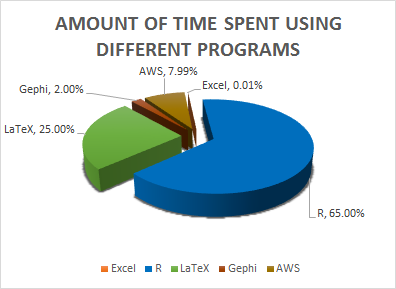
\includegraphics[width = \textwidth]{Figures/Appendix/SoftwareType}
    \caption[Software use]{Breakdown of the time used on each software type in this project.}
    \label{fig:SofwareType}
\end{figure}


\section{R Packages}
\label{sec:packages}
The Following R packages were used in this project

stringr \cite{wickham2015}, lubridate \cite{grolemund2011}, data.table \cite{dowle2015}, caret \cite{fromjedwing2016}, xgboost \cite{chen2016}, e1071 \cite{meyer2015}, R.utils \cite{bengtsson2016}, Hmisc \cite{harrelljr2016}, Matrix \cite{bates2016}, ff \cite{adler2014}, zoo \cite{zeileis2005}, networkD3 \cite{gandrud2016}, igraph \cite{csardi2006} \cite{csrdi2006}, magrittr \cite{bache2014}, ggplot2 \cite{wickham2009}, tidyr \cite{wickham2016}, xtable \cite{dahl2016}, entropy \cite{hausser2014}, dplyr \cite{wickham2016a}, microbenchmark \cite{mersmann2015}.


